\section{CONUS: Automated Validation}

ASTM E1355 Standard Guide for Evaluating the Predictive Capability of Deterministic Fire Models (2018) defines model validation as “the process of determining the degree to which a calculation method is an accurate representation of the real-world from the perspective of the intended uses of the calculation method". Model validation (“How closely do model calculations represent reality”) is assessed by comparing modeled fire perimeters to observed fire perimeters.

Obtaining the input data required for validation case studies is a cumbersome process, resulting in most models being validated against one or two fires. In many cases, historic fires are picked that the model performs well in. Some models even use optimisation and parameterisation against the historic fire they use as validation, to prove that the model has the capability of producing accurate results. This, coupled with the fact that each model chooses different historic fires and different validation metrics, makes actual validation of wildfire spread models and comparison between them almost impossible. 

To this end, Wildfire AV has been developed, the first publically available, large scale, historic wildfire validation pipeline (https://github.com/nick-cloudfire/WildfireAV). WildfireAV generates a large number of historic wildfire cases, and the input parameters required to simulate them. The pipeline creates the input files, runs ELMFIRE automatically, compares each simulation to the actual burn scar, computes similarity scores and compiles all the cases into sets for data analysis. A detailed explanation of the database, its sources, and its capabilities and limitations has been submitted for publication. 

The complete validation PDF report, comparing both ELMFIRE and FARSITE (to provide an established metric for comparison), has been included in the validation/ folder. The results are summarised here. All the results below use simple fire spread with canopy effects, no firebrands, barriers, no suppression. 

Overall, ELMFIRE seems to have a more balanced output with regards to over- or underestimation of total fire area compared to Farsite, which may be attributed to its breaching criterion (Farsite hard stops fire spread at barriers). 

\begin{figure}[h!]
    \centering
    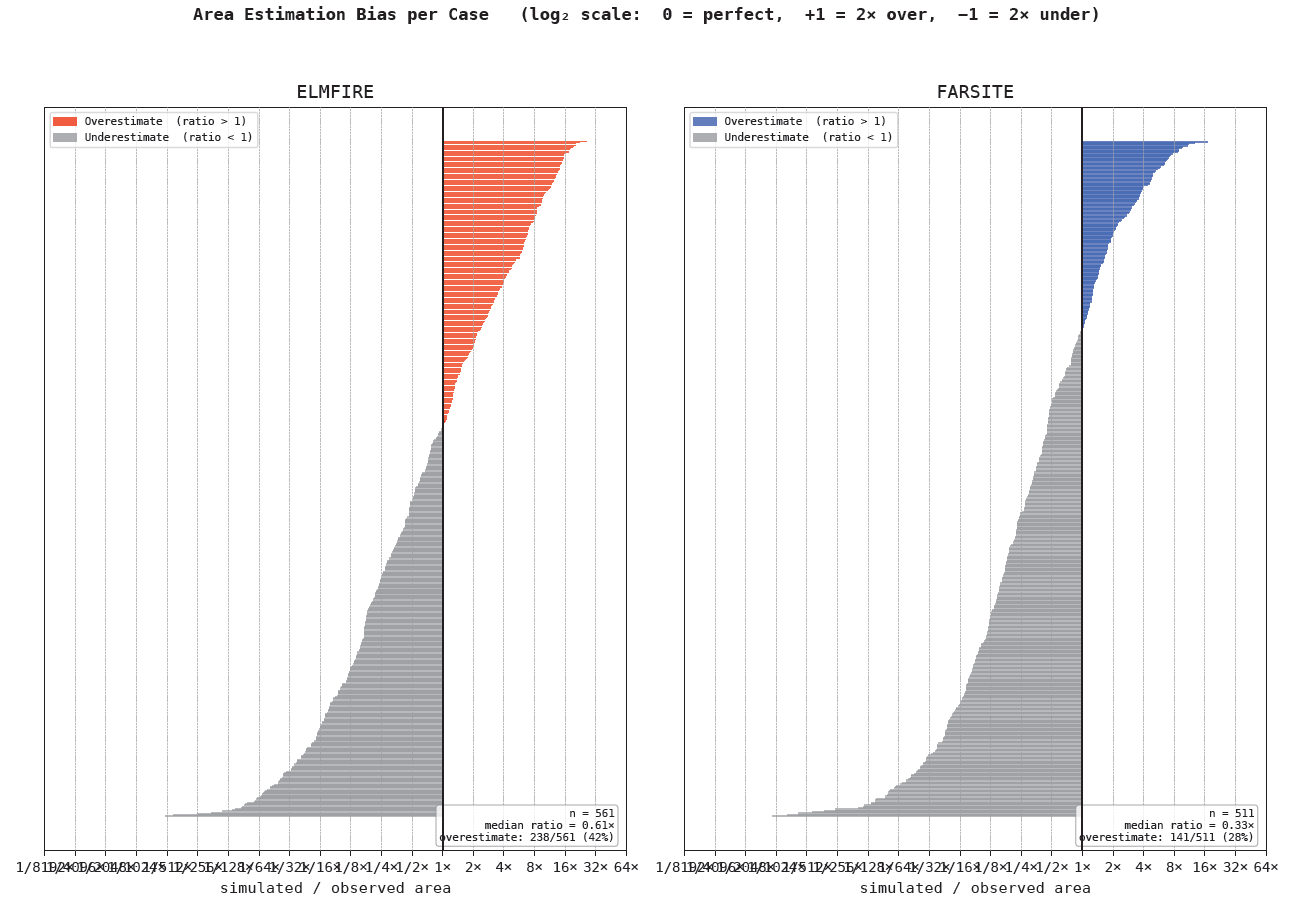
\includegraphics[width=0.75\linewidth]{figs/WAV_bias.png}
    \caption{A bias estimation plot, with the over- and underestimation of each case plotted (through simple total area comparisons.}
    \label{fig:WAV_bias}
\end{figure}

In terms of overall similarity score, ELMFIRE and Farsite obtain broadly similar scores, with ELMFIRE having a mean Jaccard coefficient of 0.178, a mean Sorensen Coefficient of 0.278 and a mean Cohen's kappa of 0.241. THe equivalent Farsite values are 0.176, 0.274 and 0.249. The distributions also look similar, with the elmfire curves generally skewing towards greater bulk similarity indices. 

\begin{figure}[h!]
    \centering
    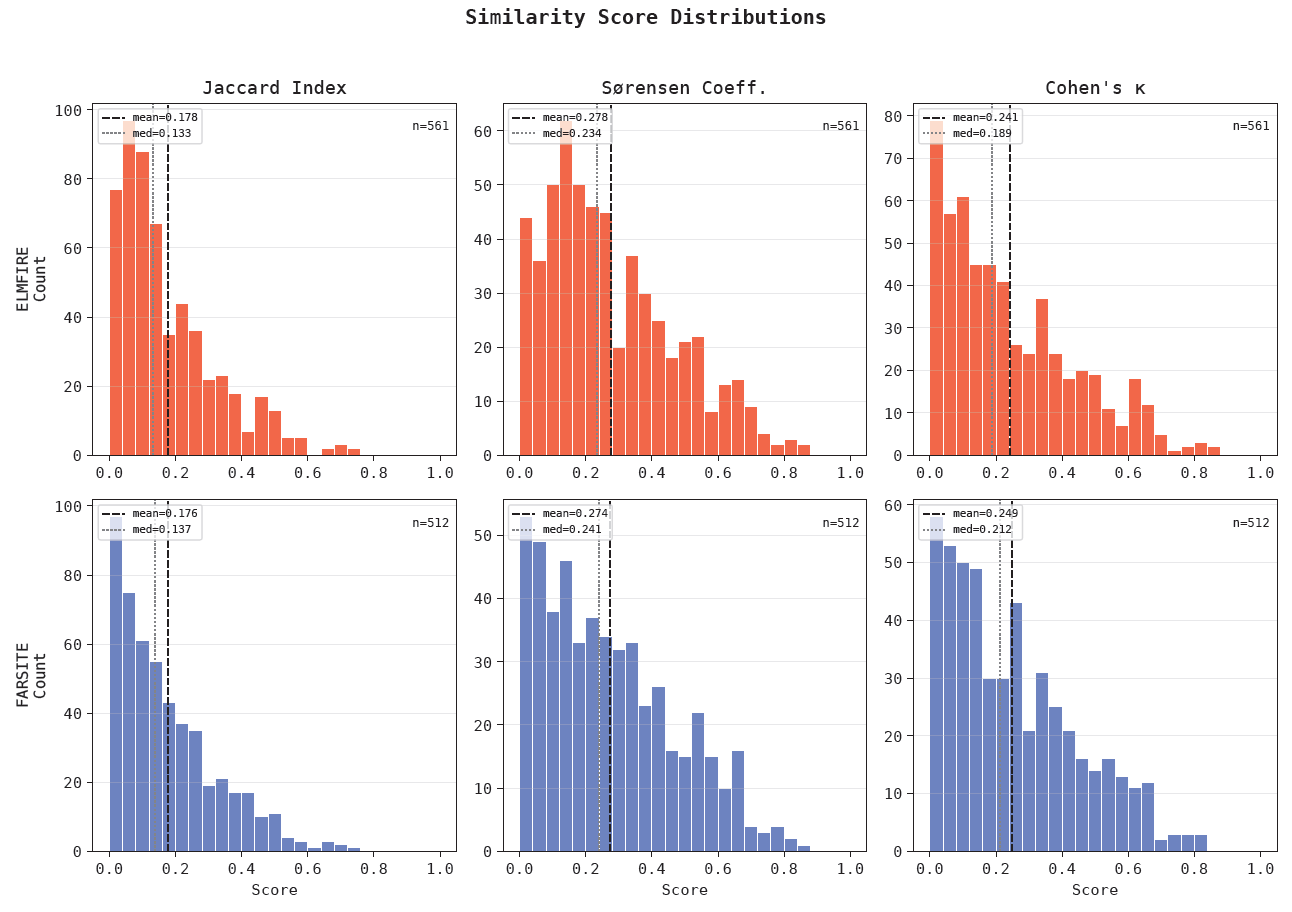
\includegraphics[width=1\linewidth]{figs/WAV_similarities.png}
    \caption{The similarity coefficient histograms of ELMFIRE and Farsite, with mean and median values superimposed.}
    \label{fig:WAV_similarities}
\end{figure}

A sample fire output is given below. For clarity, the chosen wildfire is the most accurate fire (according to its Jaccard similarity) for ELMFIRE, and shows the advantage of a conditional breaching criterion. All wildfire cases are accompanied with such a figure. 

\begin{figure}[h!]
    \centering
    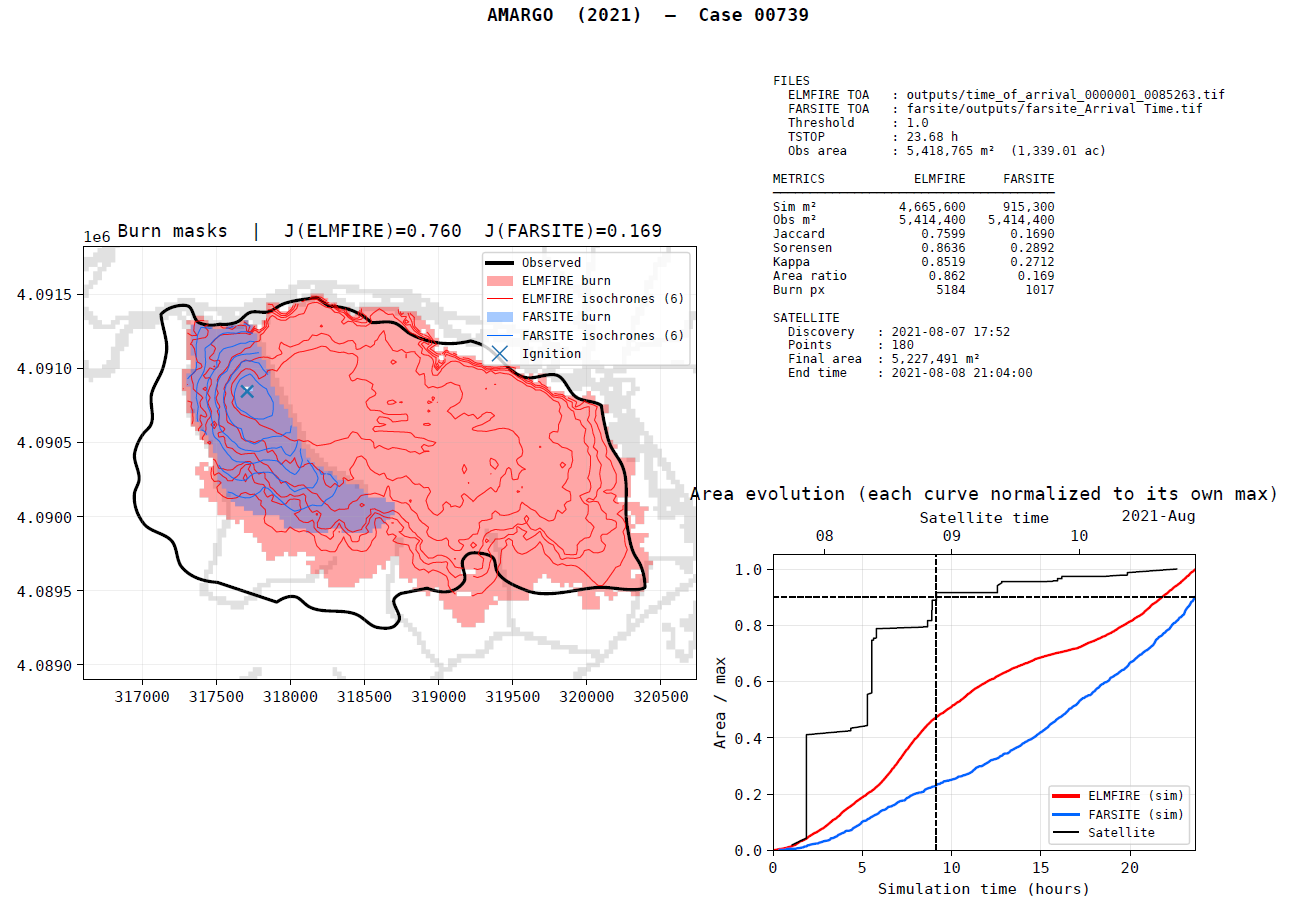
\includegraphics[width=1\linewidth]{figs/WAV_amargo.png}
    \caption{An exmaple output of a WildfireAV case, in this case the 2021 Amargo fire, the best performing ELMFIRE simulation.}
    \label{fig:WAV_amargo}
\end{figure}

Finally, for completeness, below are the top and bottom performing wildfire simulations of the dataset.

\begin{figure}[h!]
    \centering
    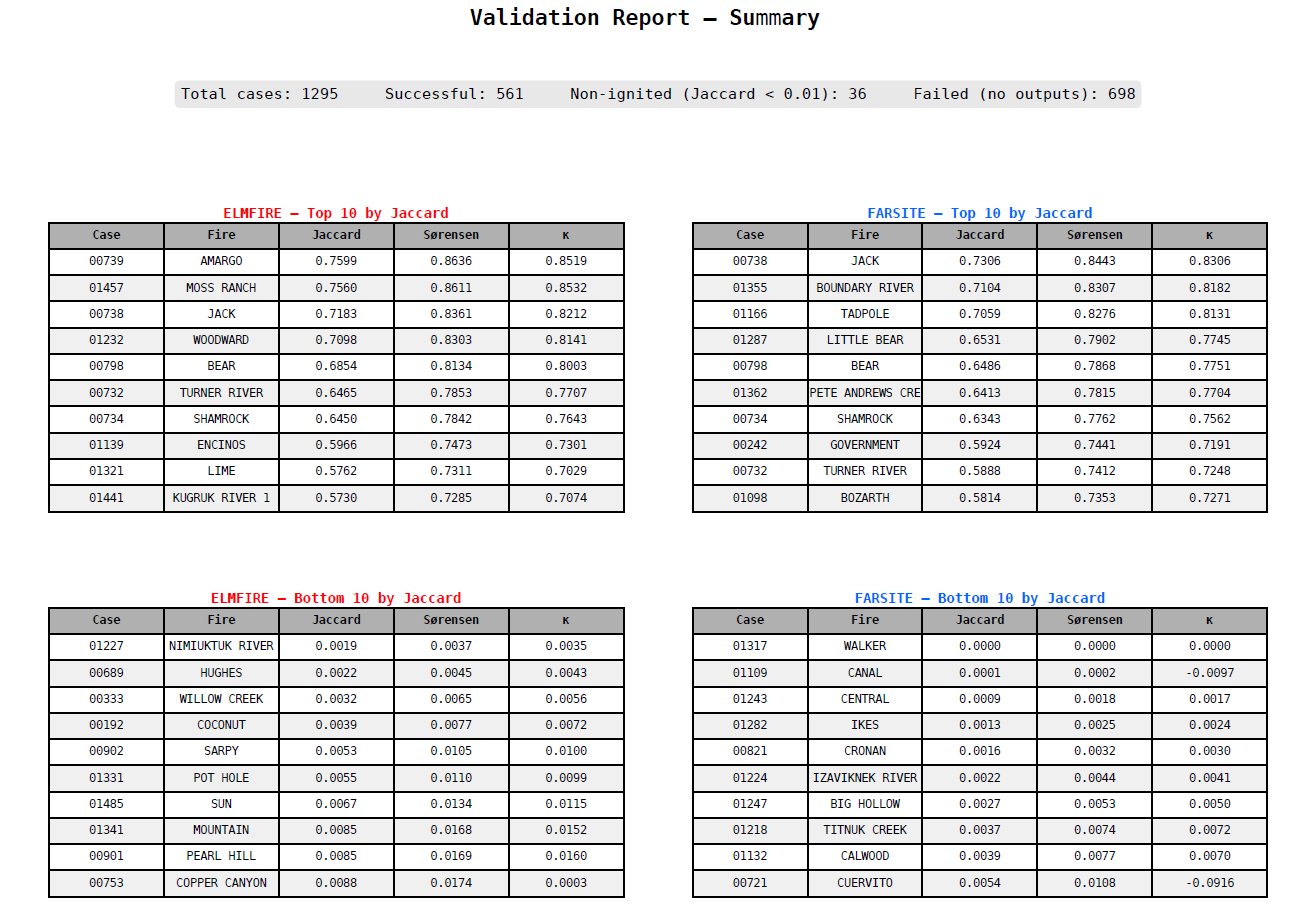
\includegraphics[width=1\linewidth]{figs/WAV_tops.png}
    \caption{The top and bottom 10 performing simulations for each model. See the full report for analytical results.}
    \label{fig:WAV_tops}
\end{figure}

\section{Canada: Dogrib Fire}

The Dogrib Fire is the standard provided validation case of the Prometheus program, the main CFFDRS fire spread model implementation \cite{tymstraDevelopmentStructurePrometheus2010}. The Dogrib fire (ID RWF085) ignited on September 25th 2001 with two main growth spurts. The first growth spurt occured between ignition and October 4th, at which point the fire was classified under control. On October 16th a wind event caused a major fire run, significantly increasing the total area of the fire. The second growth spurt of the fire was the focus of the Prometheus validation, shown in Fig. \ref{fig:dogribRealFire}, and has been recreated in ELMFIRE for the purposes of comparing the outputs of the ELMFIRE CFFDRS implementation and the real fire / Prometheus prediction. The simulation will focus on the fire spread between October 16th 13:00 local time and 19:42 local time (specified as scenario 2 in the Prometheus validation document). 

\begin{figure}
    \centering
    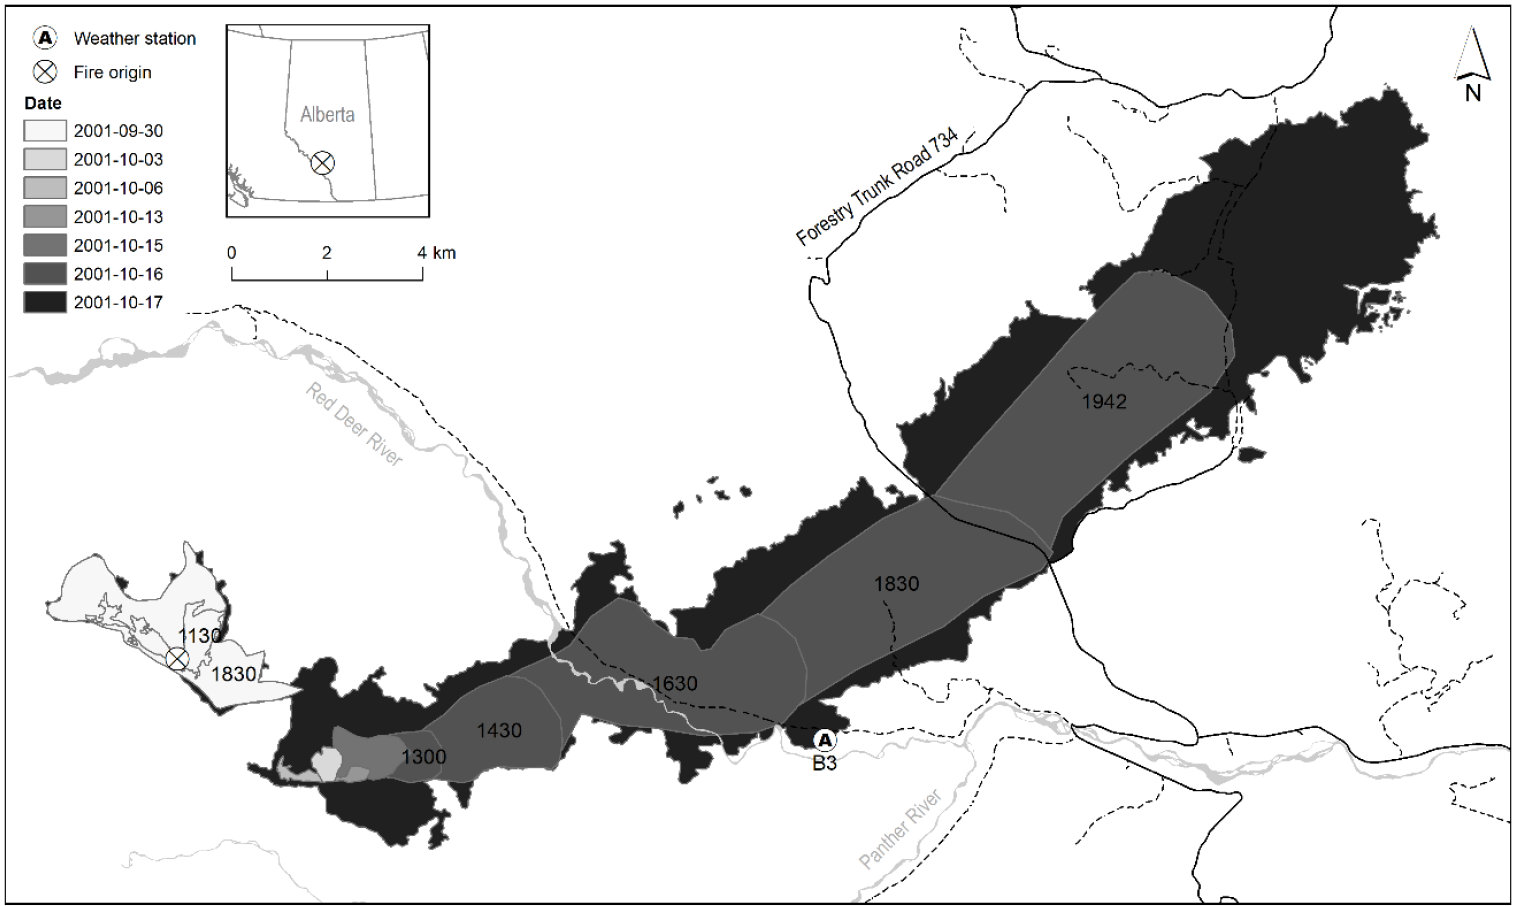
\includegraphics[width=0.8\linewidth]{figs/dogrib_real_fire.png}
    \caption{The extent and propagation of the 2001 Dogrib fire. Figure taken from the Prometheus validation supporting document "Case study information pertaining to the Dogrib sample dataset for Prometheus" by Neal McLoughlin, last revised February 3rd 2019}
    \label{fig:dogribRealFire}
\end{figure}

The supporting document of the Prometheus verification (that can be found in the Prometheus online distribution) describe the Dogrib fire extensively, along with the input data and parameters used in the simulation. The simulation used four wind scenarios:

\begin{enumerate}
    \item Weather station wind: magnitude and direction are taken directly from the local weather station. Wind magnitude is given in kilometers per hour, 10m up from vegetation canopy. Wind direction is quantized in 45 degree increments. 
    \item Modified weather station wind: wind magnitude is unchanged. Wind direction gets 15 degrees added to make the wind vector more consistent with fire spread (to account for 45 degree weather station step range). Wind is also defaulted to 280 within the river area to simulate wind channeling caused by the river valley
    \item Windninja simulation with conservation of mass, using the weather station data as inputs. 
    \item Windninja simulation with conservation of mass and momentum, using the weather station data as inputs. 
\end{enumerate}

The results with each set of wind inputs are given in detail in the Prometheus validation document, with the end result being that scenario 2 (modified weather station wind) produces the most accurate burn scar. As such, the ELMFIRE simulation will use scenario 2's wind magnitude and direction. 

In terms of the input parameters, the ones that remain unchanged between Prometheus and ELMFIRE are:
\begin{itemize}
    \item Elevation: DEM file provided in Prometheus
    \item Slope: Calculated with GDAL from the DEM file
    \item Aspect: Calculated with GDAL from the DEM file
    \item FBP Fuel Map: Provided in Prometheus
    \item Starting DMC: 64 calculated from the Prometheus weather stream
    \item Starting DC: 535 calculated from the Prometheus weather stream
    \item Ignition: Specified with coordinates in Prometheus
\end{itemize}

The following input parameters were given in the Prometheus case but had to be converted to be used in ELMFIRE:

\begin{itemize}
    \item Wind magnitude: given in the weather stream in kph, converted to mph
    \item Wind direction: taken from the weather stream and then modified in QGIS to include the weather modifications of Prometheus. 
    \item Fuel Moisture Content: Prometheus calculates Hourly Fine Fuel Moisture Code (HFFMC) from the weather stream. ELMFIRE requires fuel moisture content (1-hour) as an input. The 1-h fuel moisture content of the area can be calculated through the nelson model (as is done in the US), using the same weather stream that is provided by Prometheus. Doing so yields fuel moisture values of 18\% to 20\%. The Prometheus-derived HFFMC values translate to 9\% to 11\% fuel moisture content. For the validation case, the HFFMC-derived fuel moisture content values are used (spatially consistent). M10 and M100 are irrelevant to CFFDRS calculations and are taken from the Nelson model results.
    \item Degree of curing: Prometheus specifies 100\% degree of curing for all grass type fuels. ELMFIRE translates this input as a Live Herbaceous moisture content of 30\%.
    \item FWI Interpolation: The dogrib simulation provided with the Prometheus installation is ran with the Lawson diurnal FWI interpolation model. The Lawson model interpolates hourly fine fuel moisture code (HFFMC) and Hourly Initial Spread Index (HISI), the two most critical parameters of fire spread, from a diurnal drying and wetting profile, using the daily midday weather values. The alternative method is the Van Wagner method which relies on hourly weather values to calculate the HFFMC and HISI. The two methods offer advantages and disadvantages in their application and accuracy; their main difference is that Lawson produces a strong diurnal cooling effect whereas Van Wagner has a weak nighttime cooling effect. In the Dogrib simulation of ELMFIRE, the Lawson model is used, but ELMFIRE can only implement the Van Wagner model. As such, the simulation that is used here to represent the results of Prometheus were rerun with the Van Wagner interpolation model, to make the comparison more straightforward. 
\end{itemize}

The results of the Prometheus and ELMFIRE simulation are presented in Fig. \ref{fig:dogribSimResults} and show that ELMFIRE predicts significantly smaller fire size than Prometheus, and both models underpredict the extent of the fire. Focusing on the discrepancy between ELMFIRE and Prometheus, the difference between the two predictions can be condensed to the way the two models propagate the fire in 2D. 

\begin{figure}[h]
    \centering
    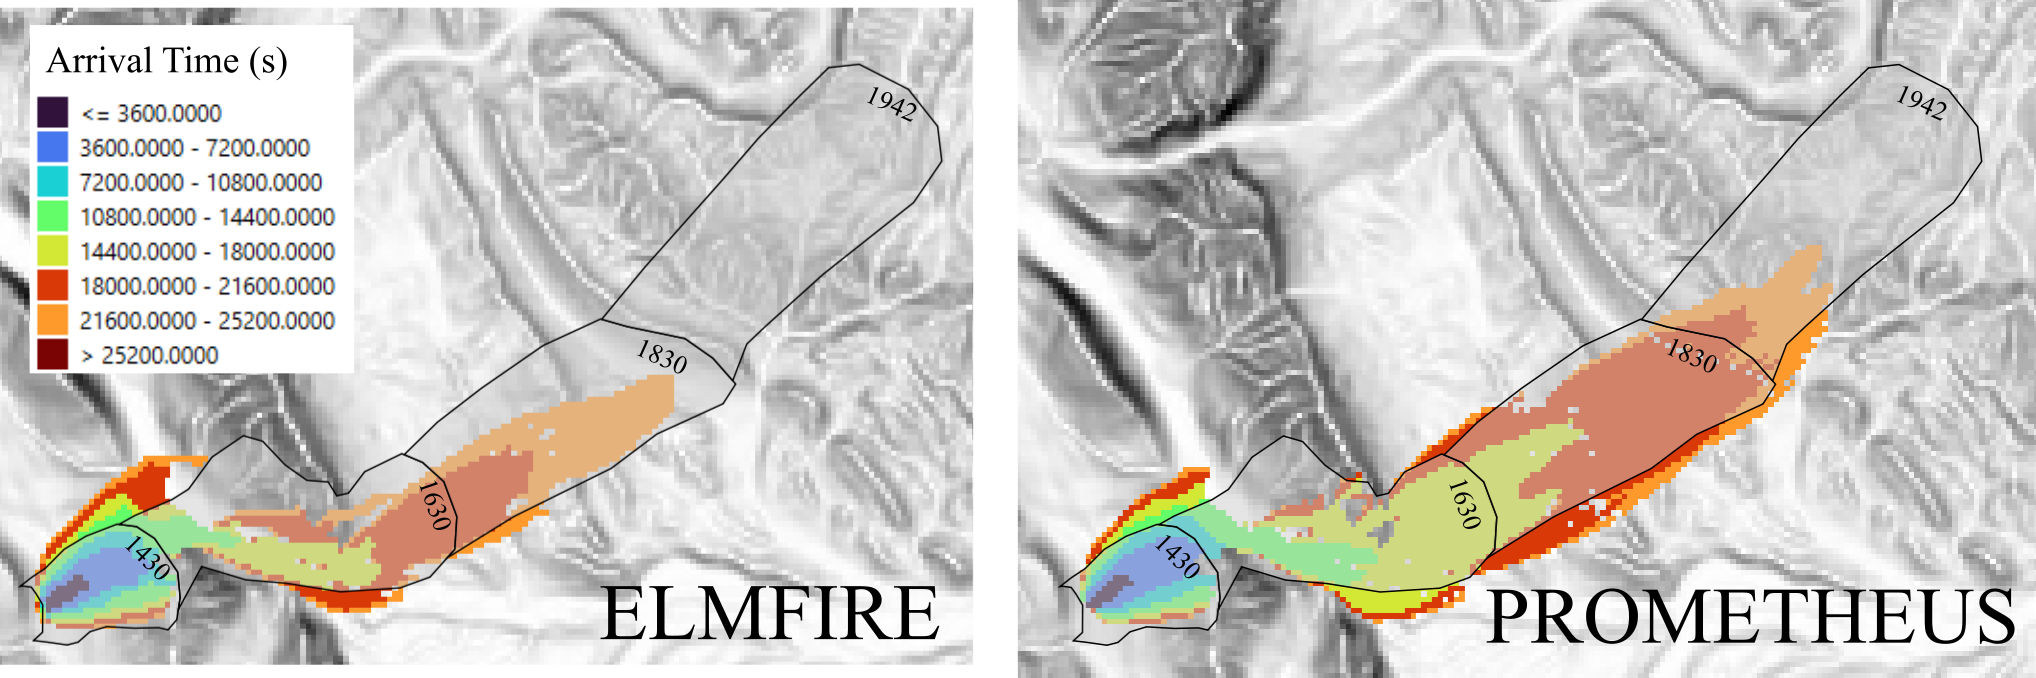
\includegraphics[width=0.95\linewidth]{figs/dogrib.png}
    \caption{The burn scars of ELMFIRE and Prometheus for the Dogrib fire with identical / parsed input parameters.}
    \label{fig:dogribSimResults}
\end{figure}

Take the example given in table 3 or the 2009 FBP Update document \cite{wottonUpdatesRevisions19922009}. For a fire with head fire rate of spread of 17.46 m/min, and a Length-to-breadth ratio of 1.98 (referring to the length to breadth ratio of the elliptical fire spread from a point source. The original document predicts a backwards rate of spread of 2.16 m/min, using the FBP methodology. ELMFIRE uses the updated methododology employed in Farsite to calculate the rate of spread in any direction. It specifically calculates the backwards rate of spread through:

\[
ROS_b=ROS\frac{LOW-\sqrt{LOW^2-1}}{LOW+\sqrt{LOW^2-1}}
\]

Plugging in the values from the update document yields a value of 1.29 m/min. This behavior can be considered a universal property of ELMFIRE and a key driver of the difference between it and Prometheus. In the dogrib simulations, a critical component of the fire spread is the transverse travel of the fire over and across the landscape ridges. Before the fire crosses the river, in particular, it has to spread on a 60 degree downhill, shown in Fig. \ref{fig:dogribCliff}, which would produce drastically different rates of spread. A comparison of multiple models in the literature \cite{kalogeropoulosWildfireSimulationsProtect2025} shows that different models treat point sources with different elliptical shapes and dimensions, and the ellipses of ELMFIRE and Prometheus are particularly different in their flank and backfires. 

\begin{figure}
    \centering
    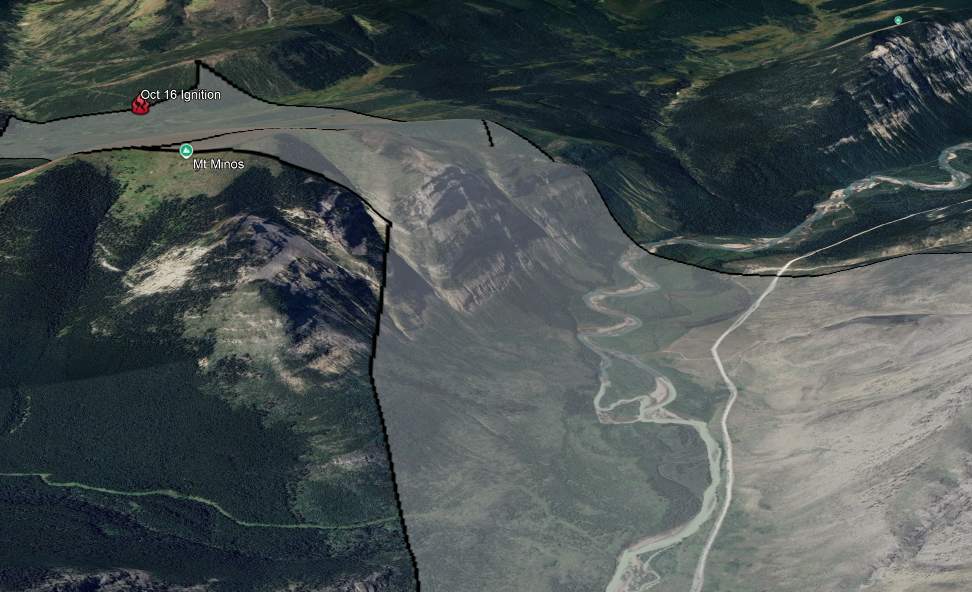
\includegraphics[width=0.75\linewidth]{figs/dogrib_cliff.png}
    \caption{The 60 degree downhill part of fire spread shown in Google Earth. It is highly likely that the fire spread of the real fire was assisted and accelerated by firebrands travelling from the top of the hill to the valley below and beyond the river. However, firebrand-assisted propagation is already reflected in the CFFDRS spread rate regressions, and as such should not be activated in ELMFIRE.}
    \label{fig:dogribCliff}
\end{figure}

To further investigate this, the Dogrib simulations were repeated, with terrain effects turned off, meaning the elevation was changed to a constant value, and the slope and aspect were both set to zero. The results depicted in Fig. \ref{fig:dogribFlatSim} show that, with only the wind pushing the fire, and thus the burn extent primarily depending on the head fire spread rate, the results are near identical (barring differences in flank fire). 

\begin{figure}[h]
    \centering
    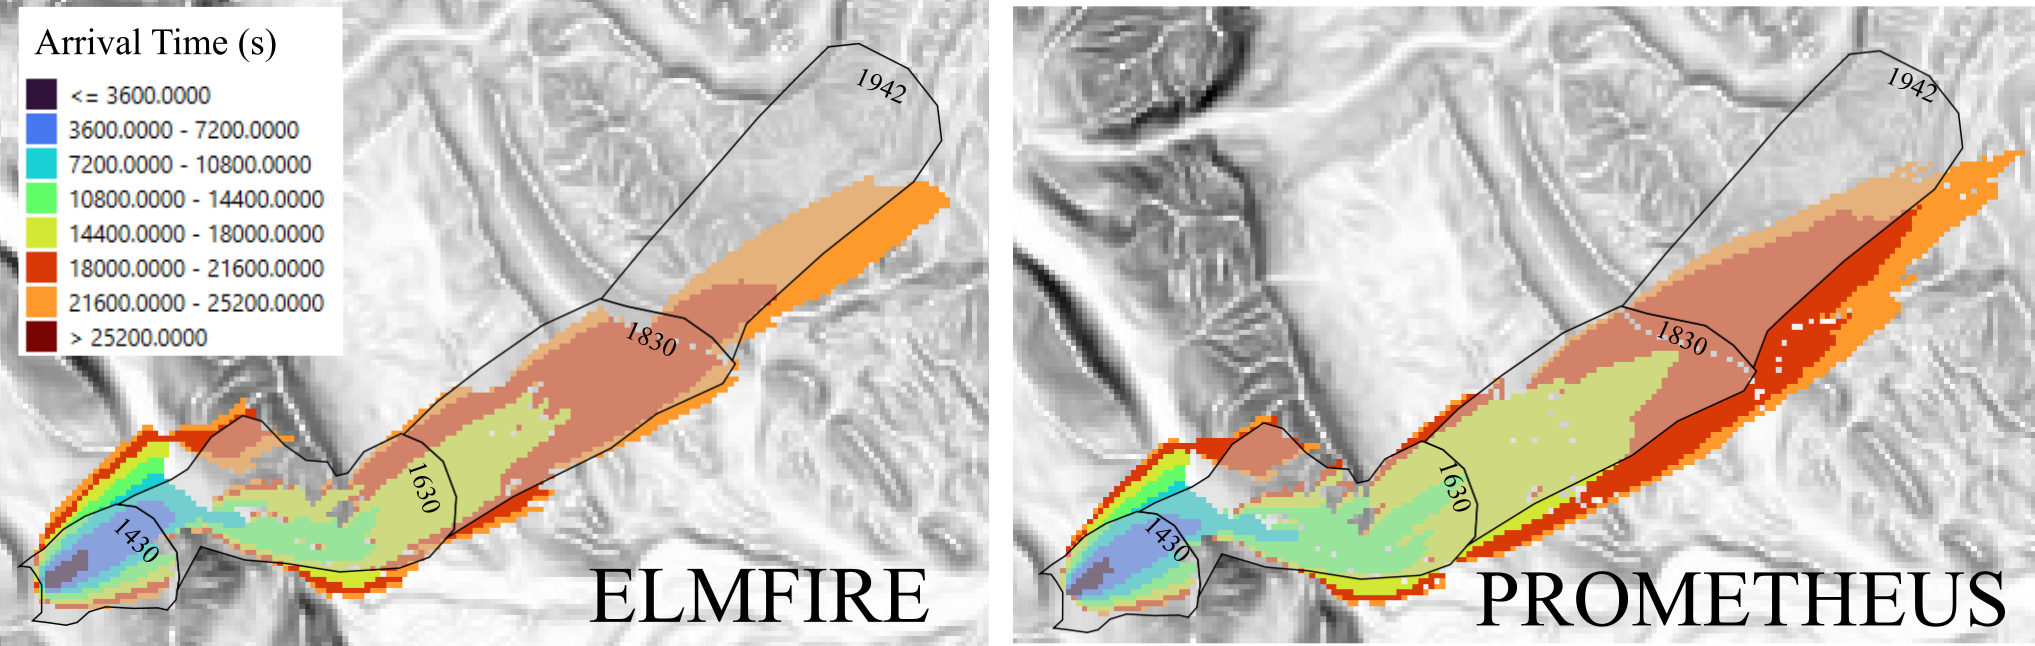
\includegraphics[width=0.95\linewidth]{figs/dogrib_flat.png}
    \caption{The Dogrib simulation case with flat terrain. Only the wind affects the fire spread direction and magnitude.}
    \label{fig:dogribFlatSim}
\end{figure}

With the above results, it is clear that ELMFIRE and Prometheus may produce different results, because of how they treat topography and wind interactions, with regards to spread rates and directional spread rate interpolation. Despite this result, the above simulations show that ELMFIRE is capable of producing similar outputs to Prometheus, closely approximating the behavior of real fires. 